\documentclass{article}

% Language setting
% Replace `english' with e.g. `spanish' to change the document language
\usepackage[english]{babel}

% Set page size and margins
% Replace `letterpaper' with`a4paper' for UK/EU standard size
\usepackage[letterpaper,top=2cm,bottom=2cm,left=3cm,right=3cm,marginparwidth=1.75cm]{geometry}

% Useful packages
\usepackage{wrapfig}
\usepackage{graphicx}
\graphicspath{ {./images/} }
\usepackage{csquotes}
\usepackage[backend=biber]{biblatex}
\addbibresource{references.bib}

\title{Talos: A Beginner's Exploration of Avionics and Telemetry for Model Rockets}
\author{Nathan D. Alspaugh, Samuel J. Correa}

\begin{document}
\maketitle

\begin{abstract}
      \noindent In any aircraft or rocket, two systems are present that are essential to any flight: the avionics and telemetry systems. The avionics system controls the flight path and thrust vectoring system, monitors the rocket's orientation, and logs data. The telemetry system is responsible for transmitting this data to the ground station. In this paper, we present Talos, a project that aims to provide a beginner's approach on designing and implementing avionics and telemetry systems for model rockets. We document the learning process to design and build Talos, from the initial planning to implementation and testing. We discuss the challenges faced, the lessons learned, and the project's future work. We hope this paper will serve as a valuable resource for students and hobbyists interested in exploring the field of avionics and telemetry for model rockets. Our results show that it is possible to design and build a functional avionics and telemetry system for model rockets using specialized components and open-source software accessible by any high school student. We believe that Talos has the potential to inspire others to explore the exciting world of aerospace engineering and rocketry.
\end{abstract}

\section{Introduction}

\qquad As dedicated students passionate about aerospace and mechanical engineering, we decided to explore these topics by building an avionics and telemetry system for model rockets. Talos, named after the mythical giant bronze automaton, is a project that aims to provide a beginner's perspective on the design and implementation of such systems. With a limited budget, space constraints, and hardware limitations, our design process was shaped by these restrictions and allowed us to think like engineers.
\section{Background Research}

\qquad Avionics refers to the electronic systems used in aircraft and spacecraft. They are responsible for navigation, communication, flight control, and monitoring. In the context of model rockets, avionics systems control the thrust vectoring system, parachute, log data, and transmit it to the ground station through telemetry. Combining Flight Control Systems, Air Data Systems, and Inertial Sensor Systems makes these avionics systems possible. Telemetry systems transmit data from the rocket to the ground station using communication transceivers.


% \begin{figure}[p]
%       \caption{Avionics Flowchart}
%       \label{fig:flowchart}
%       \centering
%       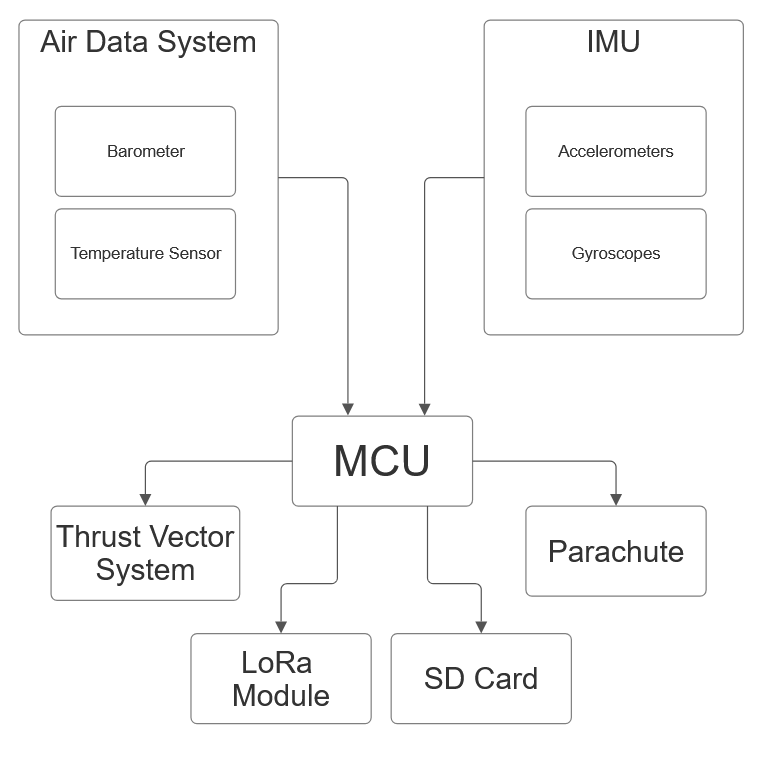
\includegraphics[width=0.75\textwidth]{flowchart.png}
% \end{figure}
The Flight Control System employed in Talos utilizes the auto stabilization (or stability augmentation) system described in \cite{Collinson_2012} and can be seen in Figure \ref{fig:flowchart}. This system uses sensors to measure the rocket's orientation and adjust the control surfaces to maintain a desired flight path.


The Air Data System measures the rocket's altitude and airspeed. It should compute these values using a combination of pressure and temperature sensors.

\newpage

\begin{wrapfigure}{l}{0.5\textwidth}
      \caption{Flight Control System}
      \label{fig:flowchart}
      \centering
      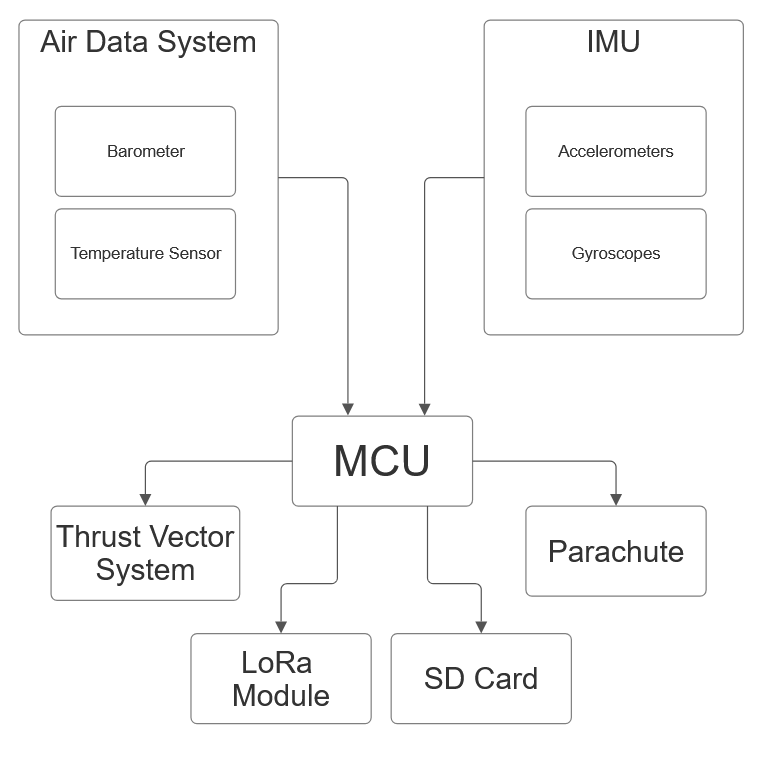
\includegraphics[width=0.5\textwidth]{flowchart.png}
\end{wrapfigure}


The Inertial Sensor System measures the rocket's orientation and acceleration. It uses sensors that can measure rotation (gyroscopes) and acceleration (accelerometers). In conjunction with the Air Data System, the INS can compute the rocket's velocity vector information.

We decided to use the LoRa (Long Range) protocol for the Telemetry System. LoRa is a long-range, low-power wireless communication protocol ideal for transmitting telemetry data from the rocket to the ground station. The LoRa protocol, based on spread spectrum modulation techniques, increases reliability by "spreading" the signal over more frequencies and can transmit data over long distances (up to 10 km) with low power consumption. These factors make LoRa ideal for model rockets, where power consumption and range are critical factors. It is also very immune to the Doppler effect\cite{8723123}, which is important for rockets moving at high speeds.
\newline
\section{Methodology}

\qquad We divided the Talos project into planning, design, implementation, and testing phases. Each phase involved a series of tasks and challenges that must be solved.

\subsection{Planning}

\qquad The planning phase involved defining the project scope, setting goals, and identifying the components needed. We started by researching existing avionics systems and telemetry solutions to understand the requirements and challenges. We then defined the key features of Talos, such as flight control, telemetry, and data logging. We also identified the components needed, such as sensors, microcontrollers, and communication modules. Our goal was to make a flight controller with dimensions 12 cm x 5 cm, with a USB-C port an headers for the thrust vectoring system and parachute deployment.
\subsubsection{Breakout Board or Custom Printed Circuit Board (PCB)?}
\qquad After thorough research, we designed our custom PCB for the Talos project. Heavily impacted by the rocket's space constraints and the need for a powerful microcontroller with custom sensors, typical breakout boards (Arduino or ESP32 based) were insufficient for our use. When we started the project, we had no experience with PCB design, so we had to learn how to use EasyEDA, a free online PCB design tool.
\subsubsection{Microcontroller Selection}
\qquad We decided to use the STM32F405 microcontroller for the Talos project. Particular CubeSat projects have also been using the STM32 Family\cite{Yost_2023}, which affected our decision in selecting the microcontroller.We chose this microcontroller because of its speed and versatility (see Figure \ref{fig:microcontrollers}) and the availability of development tools and libraries.
\begin{figure}[p]
      \caption{Table of STM32 Microcontrollers\cite{STM32_Table}}
      \label{fig:microcontrollers}
      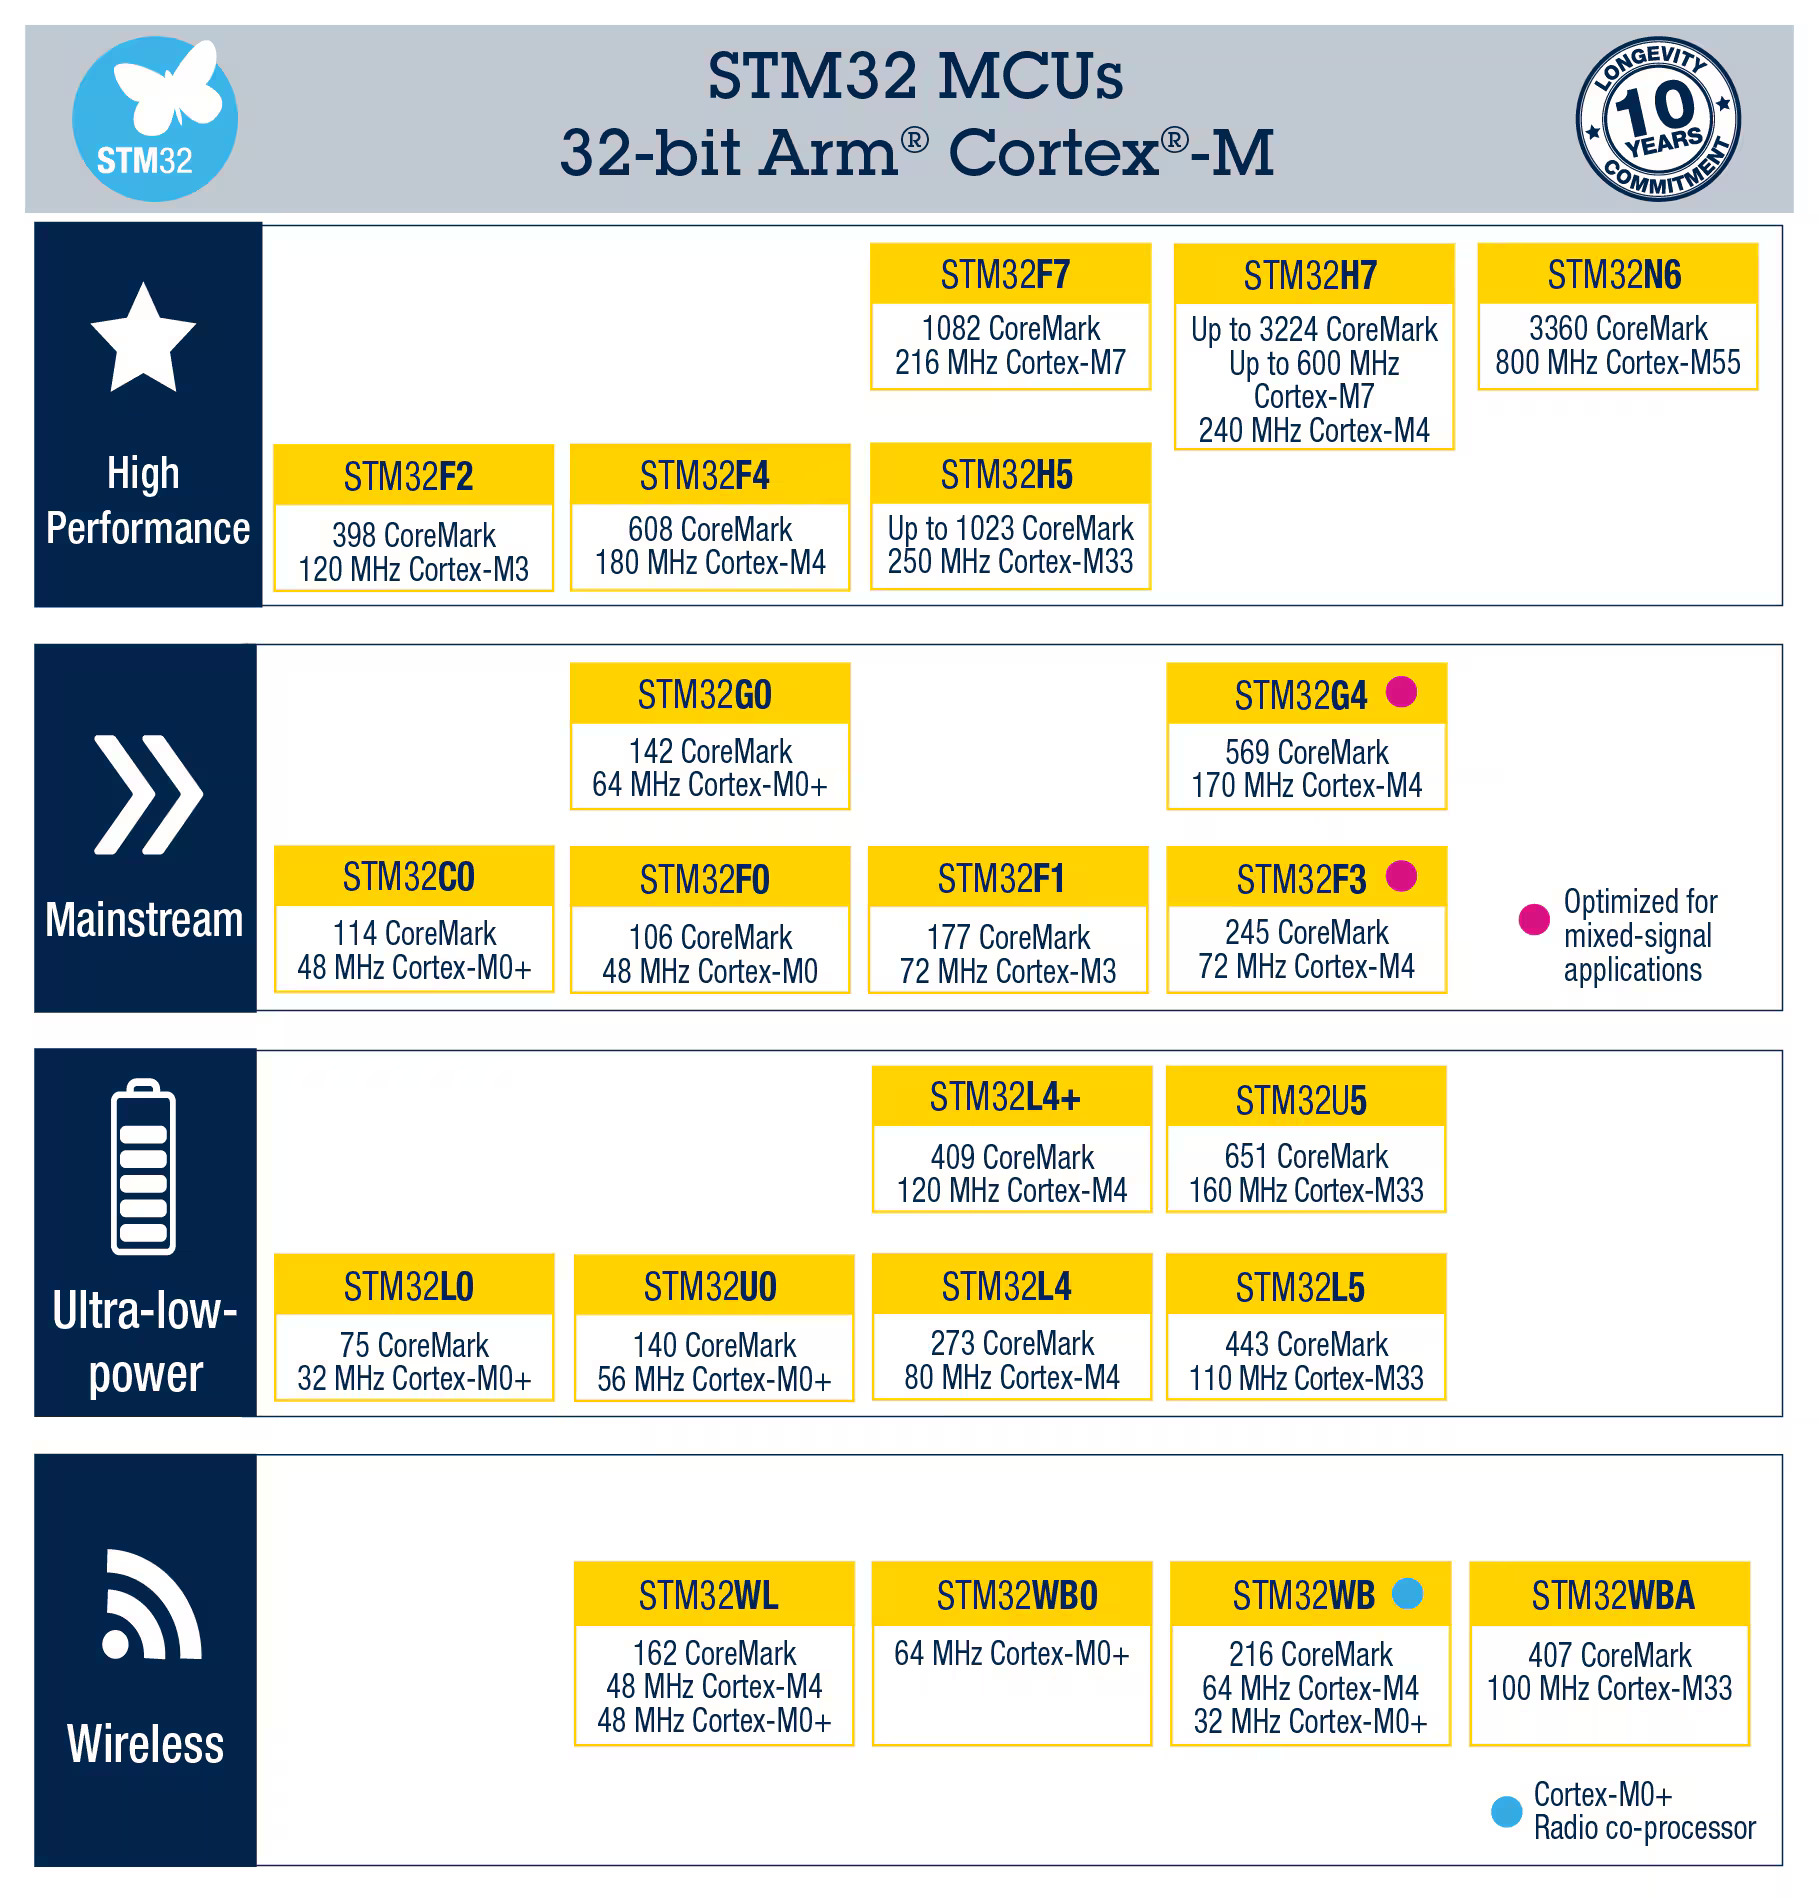
\includegraphics[width=\textwidth]{stm_mcu_chart.jpg}
      \centering
\end{figure}

\subsubsection{Sensor Selection}
\subsubsection*{Inertial Measurement Unit (IMU)}
\qquad We decided to utilize the LSM6DM IMU sensor for the Talos project. This sensor combines a 3-axis accelerometer and a 3-axis gyroscope in a single package. The LSM6DM is a MEMS (Microelectromechanical Sensor) capable of measuring acceleration and angular velocity in all three axes (see Figure \ref{fig:lsm6dm}), making it ideal for measuring the rocket's orientation and acceleration. It also includes a thermometer to measure the temperature inside the avionics and telemetry bay.
\begin{figure}[p]
      \caption{LSM6DM IMU Sensor\cite{LSM6DSM}}
      \label{fig:lsm6dm}
      \centering
      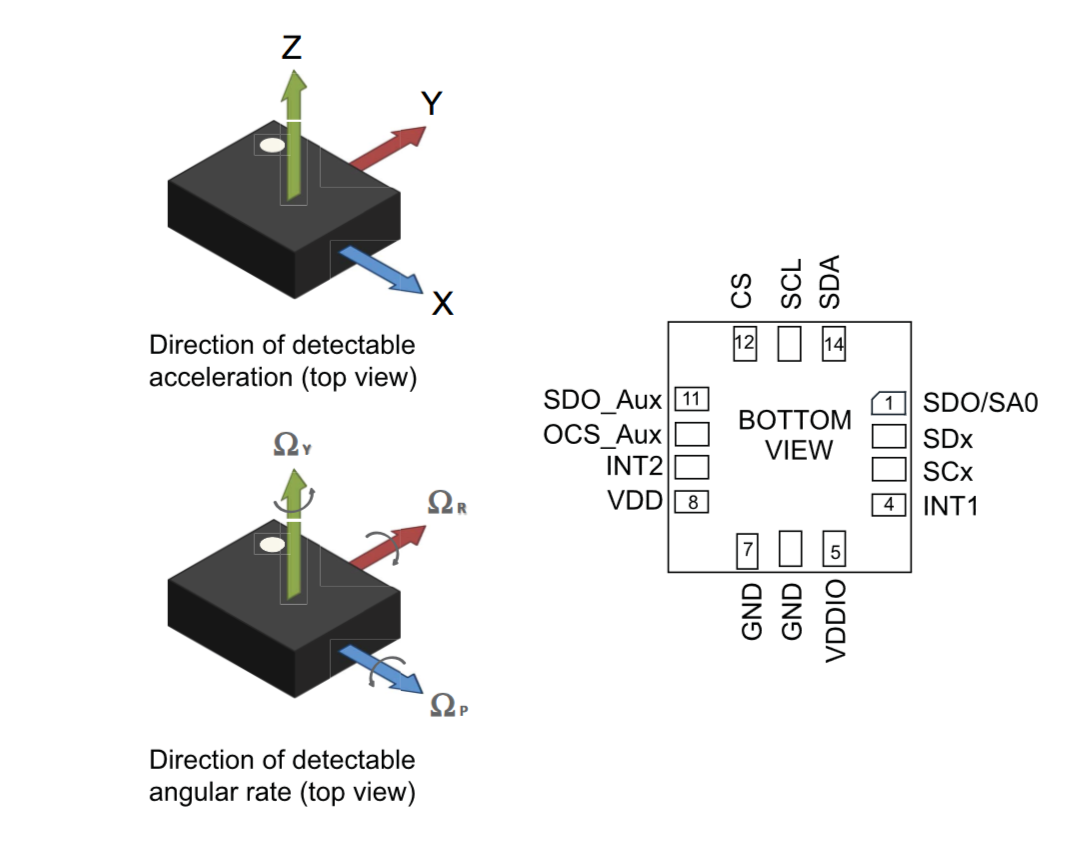
\includegraphics[width=\textwidth]{ldsm6m.png}
\end{figure}
\subsubsection*{Pressure Sensor}
For the pressure sensor, we decided to use the BMP580 (see figure \ref{fig:bmp580}).
\begin{figure}[p]
      \caption{BMP580 Pressure Sensor\cite{BMP580}}
      \label{fig:bmp580}
      \centering
      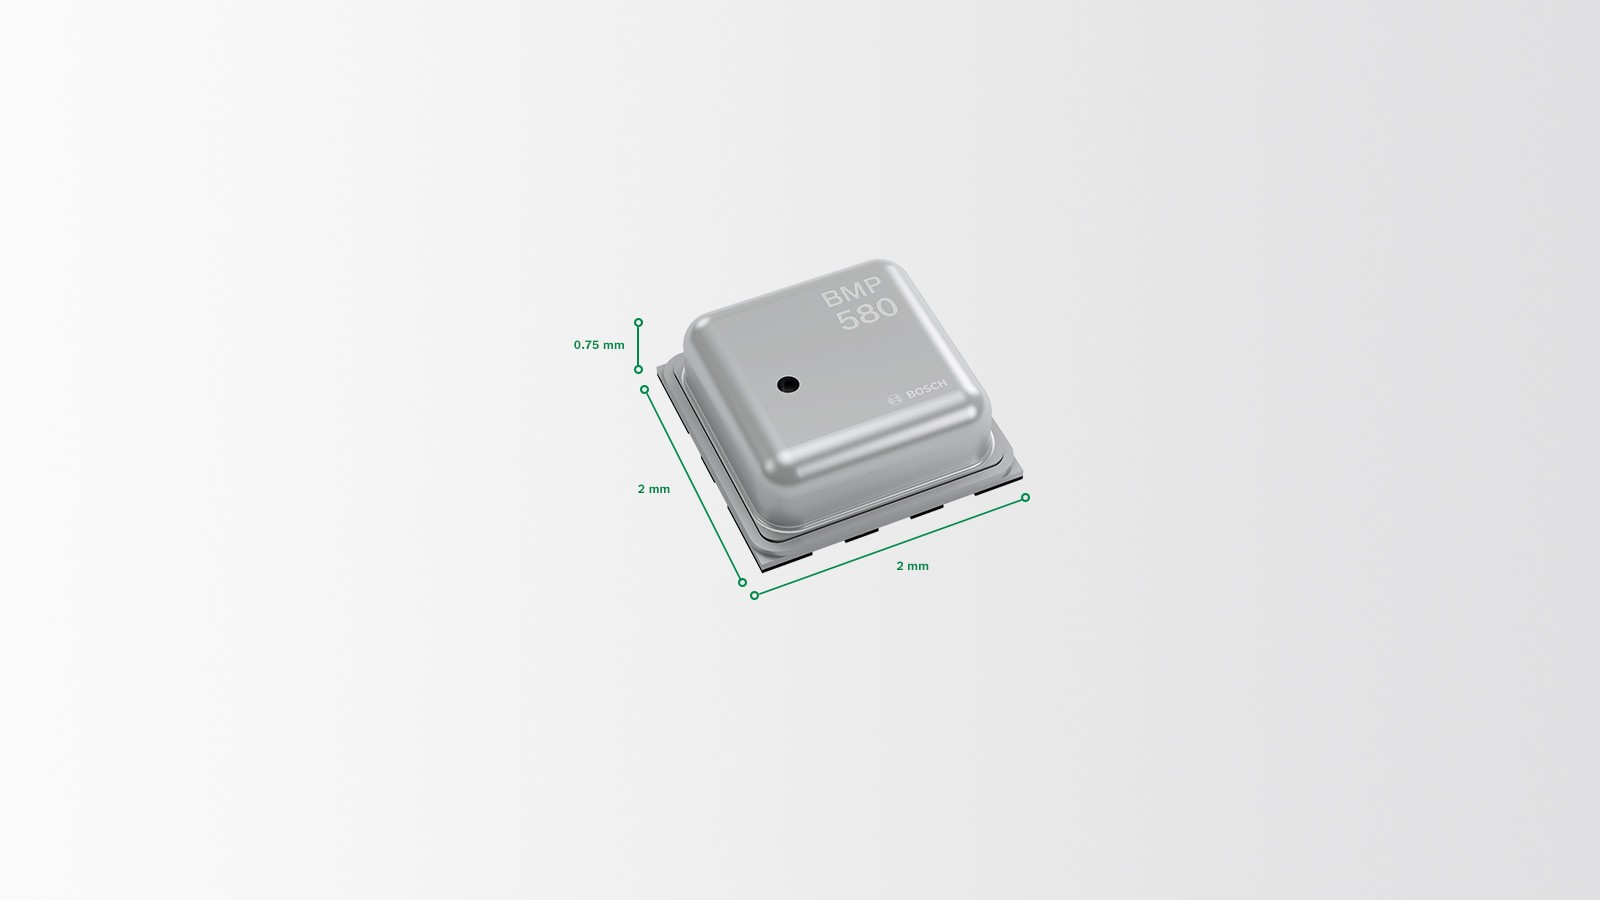
\includegraphics[width=\textwidth]{bmp580.jpg}
\end{figure}This sensor can measure pressure and temperature, which we use to calculate the rocket's altitude and airspeed. It is also more accurate than the more commonly used BMP280.\cite{Bosch_Sensortec_2024}

\subsubsection{Communication Module}
\qquad We decided to use the LLCC68 LoRa module and, more specifically, the DL-LLCC68-S-433 module for the telemetry system. We use this module specifically because of it's ease of implementation and readily available drivers that we can interface with the MCU. THe LLCC68 module also allows us to communicate at a distance with reasonable power efficiency.

\subsection{Design}

\qquad After meticulously choosing parts, we decided to embark on the design phase. This phase involved creating the schematics and PCB layout for Talos. We started by designing the schematics in EasyEDA, which involved connecting the microcontroller, sensors, and communication modules. Creating the schematics was a massive challenge as we did not know how or where to connect each sensor. We had to learn how to read datasheets and understand the electrical characteristics of each component. Taking into account Figure \ref{fig:lsm6dm}, we knew the basics of electronics: GND means ground, and VDD means power, but the other pins were a complete mystery. Here are some terms that we had to learn:
\begin{itemize}
      \item Resistor: A resistor is a passive two-terminal electrical component that implements electrical resistance as a circuit element.
      \item Capacitor: A capacitor is a passive two-terminal electrical component that stores electrical energy in an electric field.
      \item Serial Peripheral Interface (SPI): a way to communicate between devices along a single data line. Imagine it like a bus, where each device is the stop and the data is the passengers. We select the stop using the Chip Select (CS) line and then send or receive the date through the MOSI and MISO lines (SDO and SDA). The clock synchronizes the data and ensures the bus arrives when the passengers are ready to board.
            \subitem SDO: Serial Data Out
            \subitem SDA: Serial Data In
            \subitem SCL: Serial Clock
            \subitem CS: Chip Select
      \item Inter-Integrated Circuit (I2C): a way to communicate between devices along a single data line. Using the same analogy as above with the bus, the driver does not know the directions of the stops and has to ask the passengers where to go. The SDA line sends and receives data, while the SCL line synchronizes the data.
            \subitem SDA: Serial Data
            \subitem SCL: Serial Clock
      \item Interrupts: a way to notify the microcontroller that an event has occurred. These interrupts are like a bell that rings when the bus arrives at the stop.
      \item Universal Asynchronous Receiver-Transmitter (UART): a way to communicate between devices using two data lines. UART is a high speed communication protocol where data can be both sent and received at the same time. The TXD line sends data, while the RXD line receives data.
            \subitem TXD: Transmit Data
            \subitem RXD: Receive Data
      \item Pull-up and Pull-down resistors: resistors that set the default state of a pin. Pull-up resistors set the default state of a pin to high, while pull-down resistors set the default state of a pin to low.
      \item Coupling capacitors: capacitors that filter out noise in a circuit. Pull-up capacitors filter out noise in a high state, while pull-down capacitors filter out noise in a low state.
      \item Decoupling capacitors: capacitors that filter out noise in a circuit. These capacitors filter out noise in the power supply.
      \item Cross-talk: a phenomenon where signals from one circuit interfere with those from another. This cross-talk can cause errors in the data transmission.
\end{itemize}
\begin{figure}[h!]
      \caption{Talos PCB Layout}
      \label{fig:talos_pcb_layout}
      \centering
      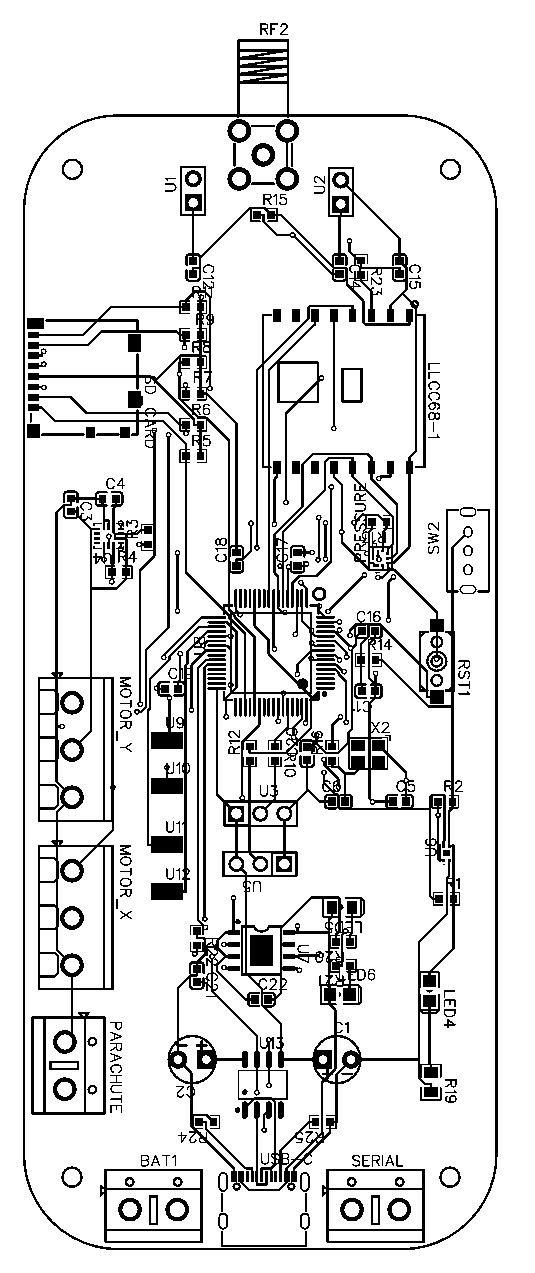
\includegraphics[width=0.5\textwidth]{PCB.png}
\end{figure}
\begin{figure}[h]
      \caption{Talos Microcontroller Schematic}
      \label{fig:talos_microcontroller_schematic}
      \centering
      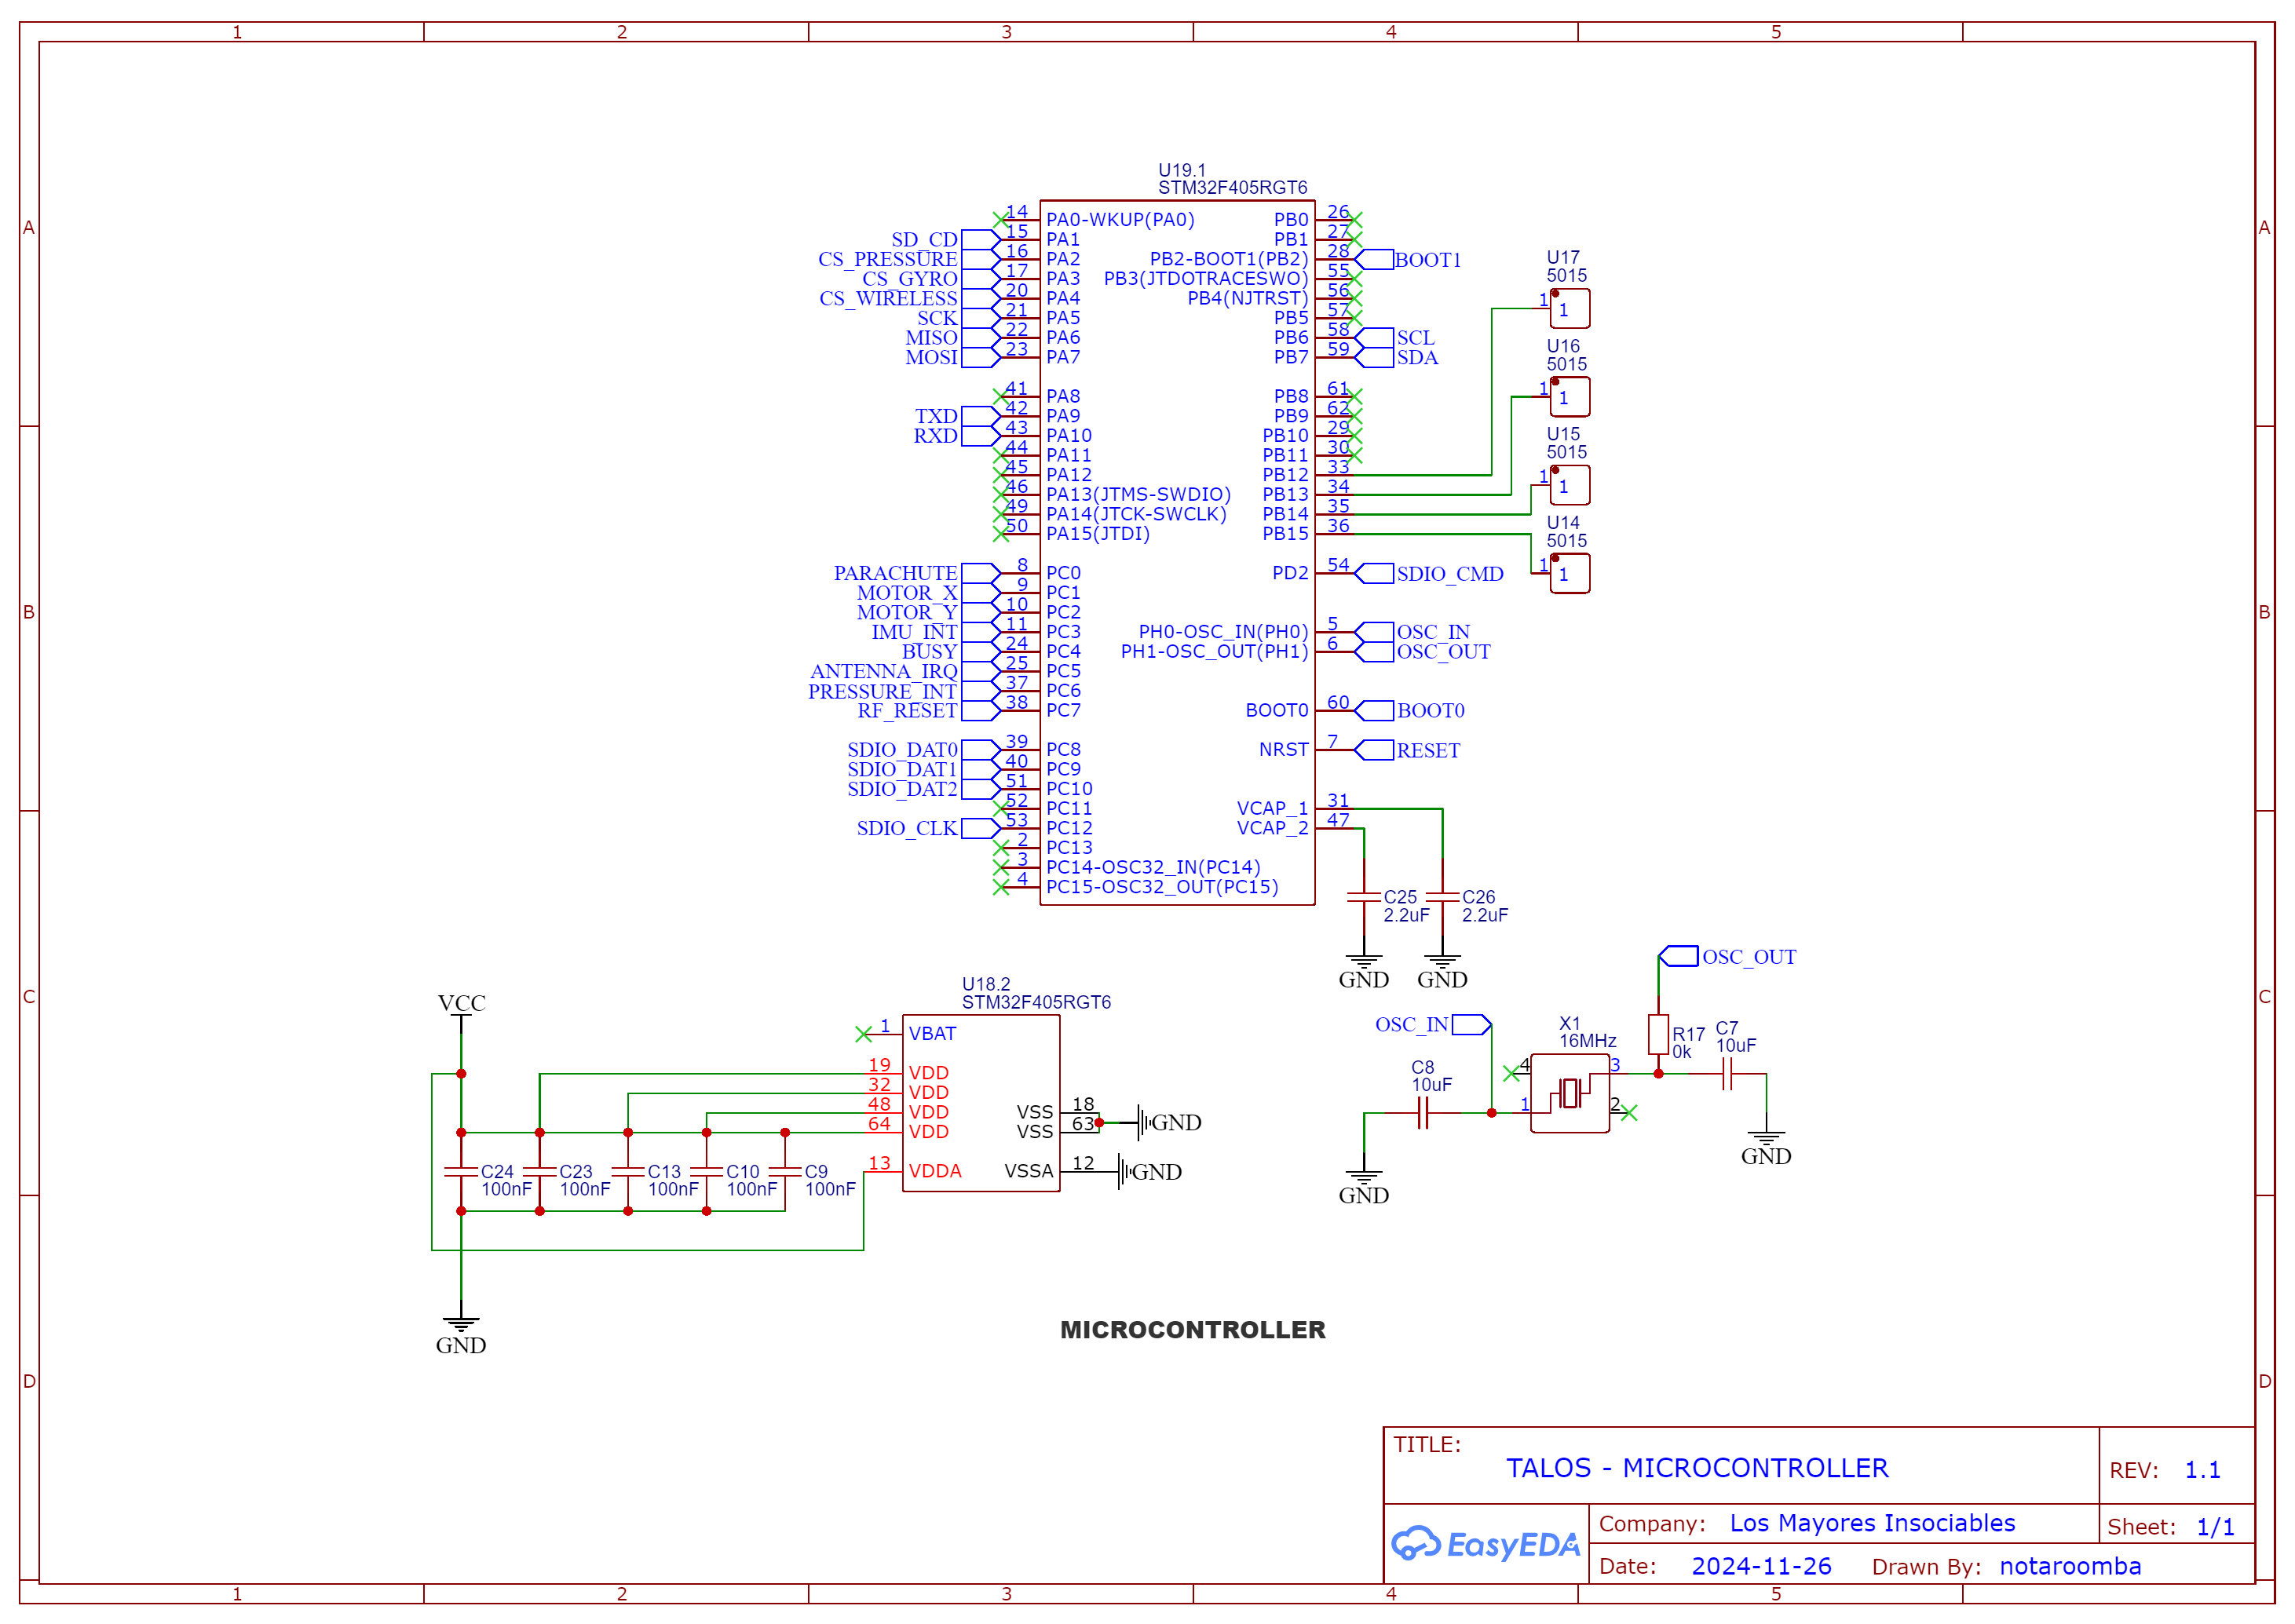
\includegraphics[width=\textwidth]{Microcontroller.png}
      \caption{Talos I/O Schematic}
      \label{fig:talos_io_schematic}
      \centering
      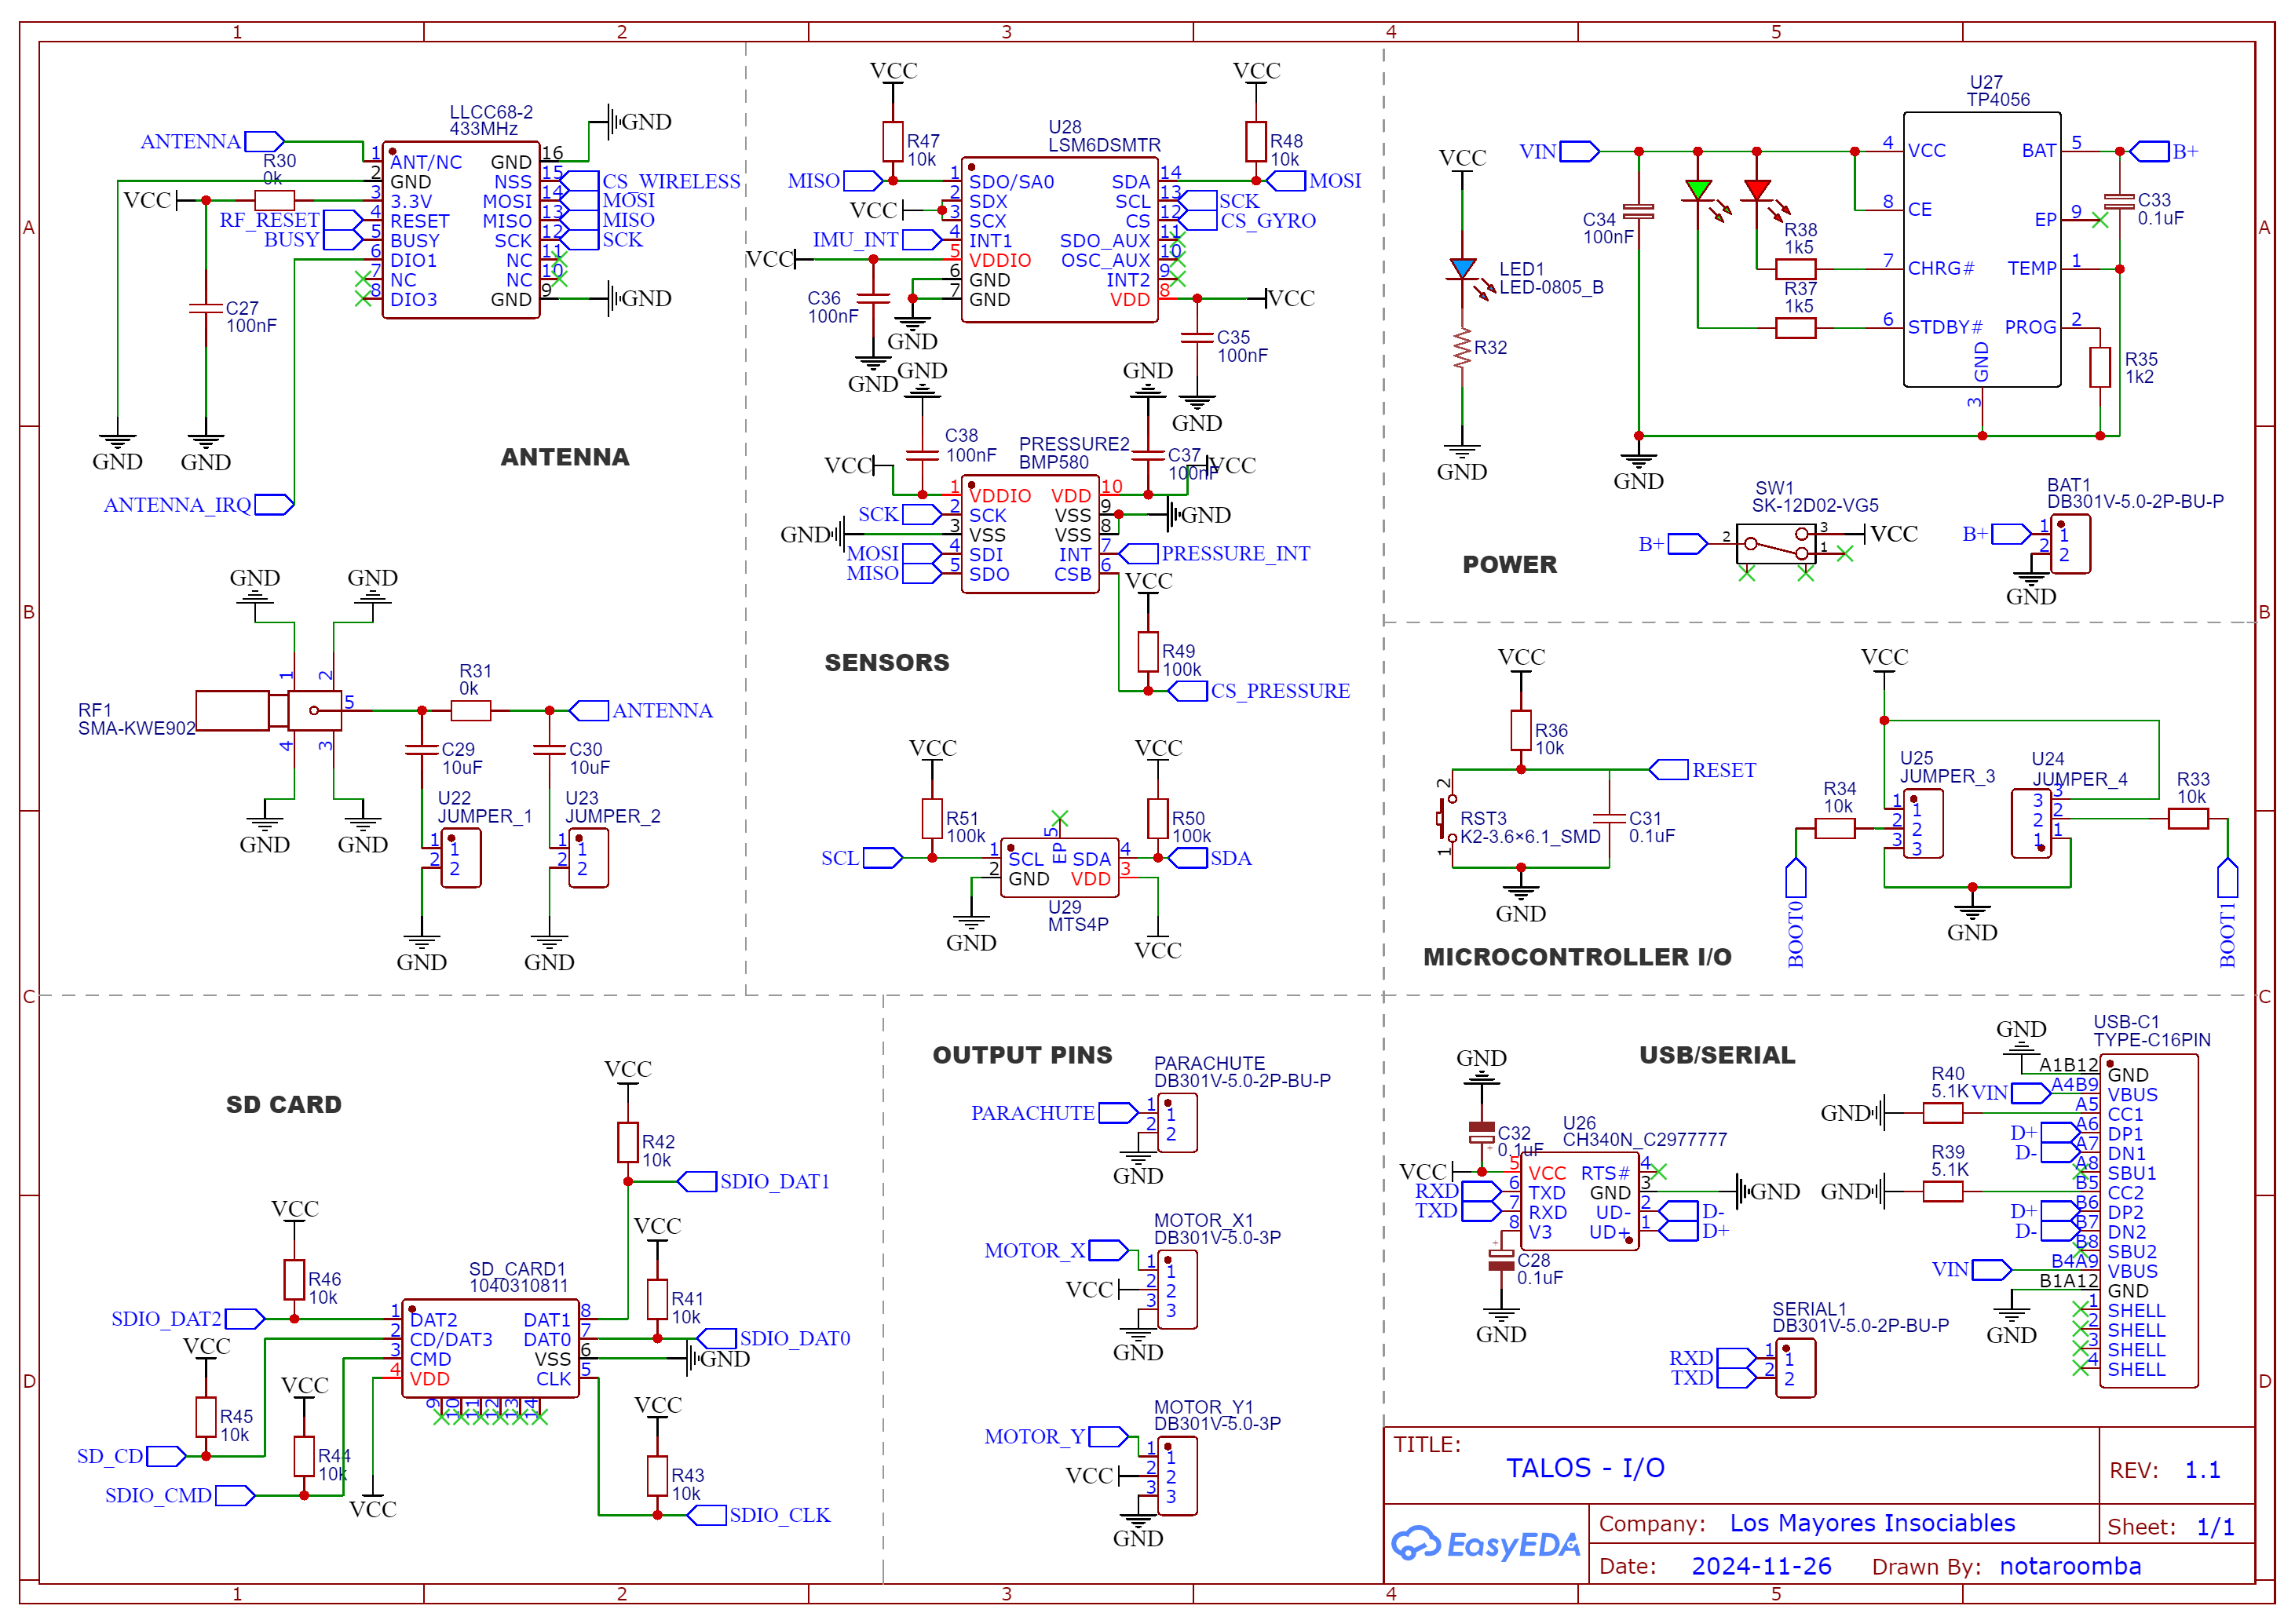
\includegraphics[width=\textwidth]{IO.png}
\end{figure}
Finally, after reading all the datasheets for each component, we created the schematic for the Talos project. Figure \ref{fig:talos_microcontroller_schematic} shows the microcontroller schematic, while the I/O schematic is at FIgure \ref{fig:talos_io_schematic}.

\subsubsection{PCB Layout}
\qquad After designing the schematics, we moved on to the PCB layout. The layout involved placing the components on the board and routing the traces to connect them. We had to consider signal integrity, power distribution, and thermal management factors. We also had to ensure that the board was compact enough to fit inside the rocket. The design was a challenging task as we had to learn how to use the PCB design software and understand the constraints of the board. We had to learn how to route traces, place components, and not make any mistakes (which we did). Here is the final PCB layout for the Talos project (see Figure \ref{fig:talos_pcb_layout}).


We decided to put the microcontroller in the center of the board, with the sensors and communication modules around it. This placement minimizes the length of the traces and reduces the risk of interference. We also added decoupling capacitors near the power supply pins of each component to filter out noise. We also added pull-up and pull-down resistors to set the default state of the pins. Finally, we added a USB-C port for programming and debugging the board. Along the sides, we took out pins to control the parachute and vector thrusting system. We also added a battery connector to power the board with a 3.3V battery. We exposed the serial lines to program directly the MCU if the USB-C port failed.

\subsection{Implementation}
\qquad After designing the PCB, we moved on to the implementation phase. This phase consisted of ordering the PCB through JLCPCB and later programming the board. Although we talked with various professors before sending the board to be made, we still made small but critical errors. When we first received the board, we encountered the following errors: firstly, the microcontroller would not turn on, and secondly, we accidentally double-switched the serial lines. In the USB/Serial section in the schematic in Figure \ref{fig:talos_io_schematic}, there is a chip with the label CH340N. This chip is responsible for the USB to Serial conversion. Part of that serial conversion is swapping the lines RXD and TXD because the USB output is the microcontroller's input. After reading the datasheet more carefully, we discovered that we crossed the lines on the CH340N chip as on the microcontroller, which resulted in the faulty USB-C port. We also missed two decoupling capacitors that were essential for a correct boot-up of the chip. The board booted up correctly after soldering the capacitors and crossing the RXD/TXD pins.
\begin{figure}[h]
      \caption{Website with no data}
      \label{fig:website_no_data}
      \centering
      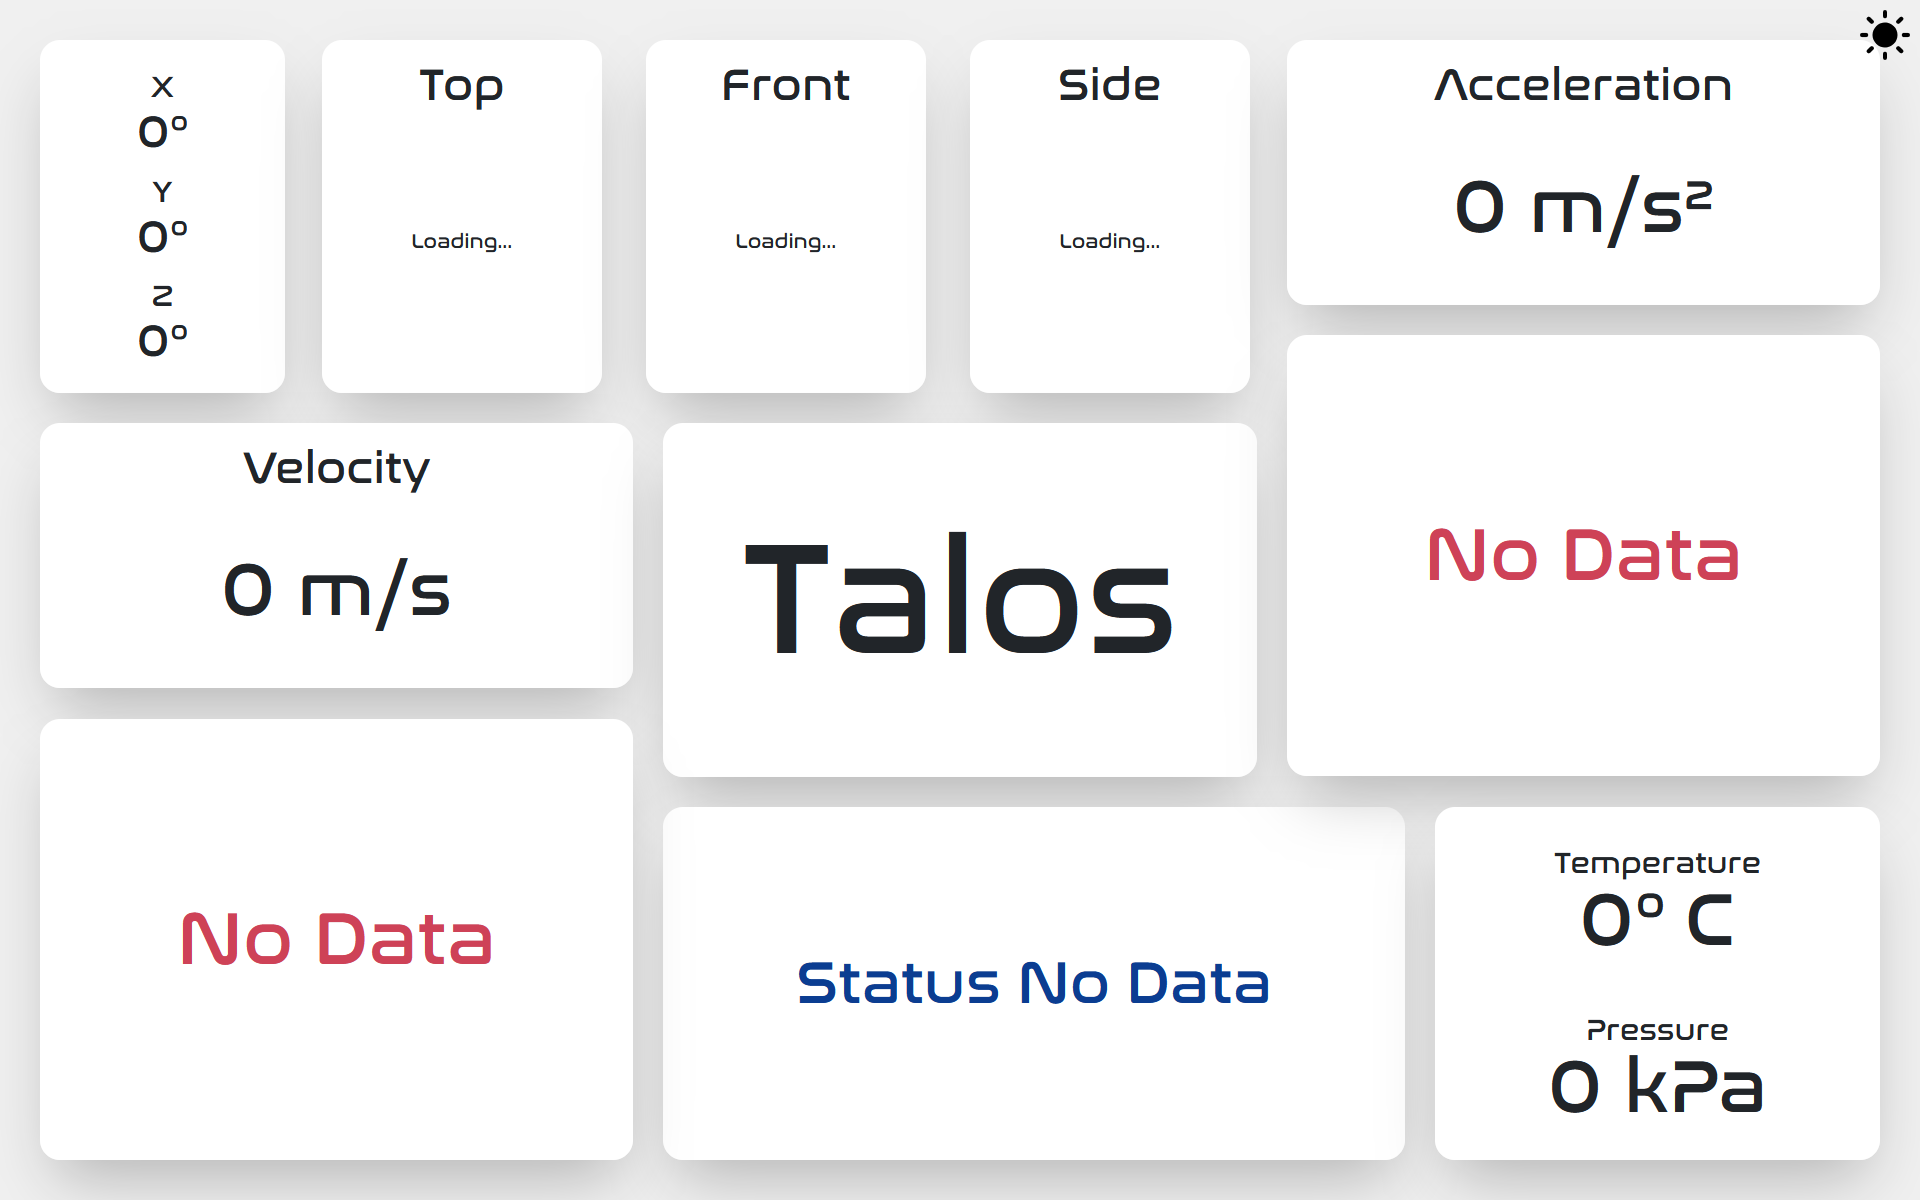
\includegraphics[width=\textwidth]{website_no_data.png}
      \caption{Website with data}
      \label{fig:website_data}
      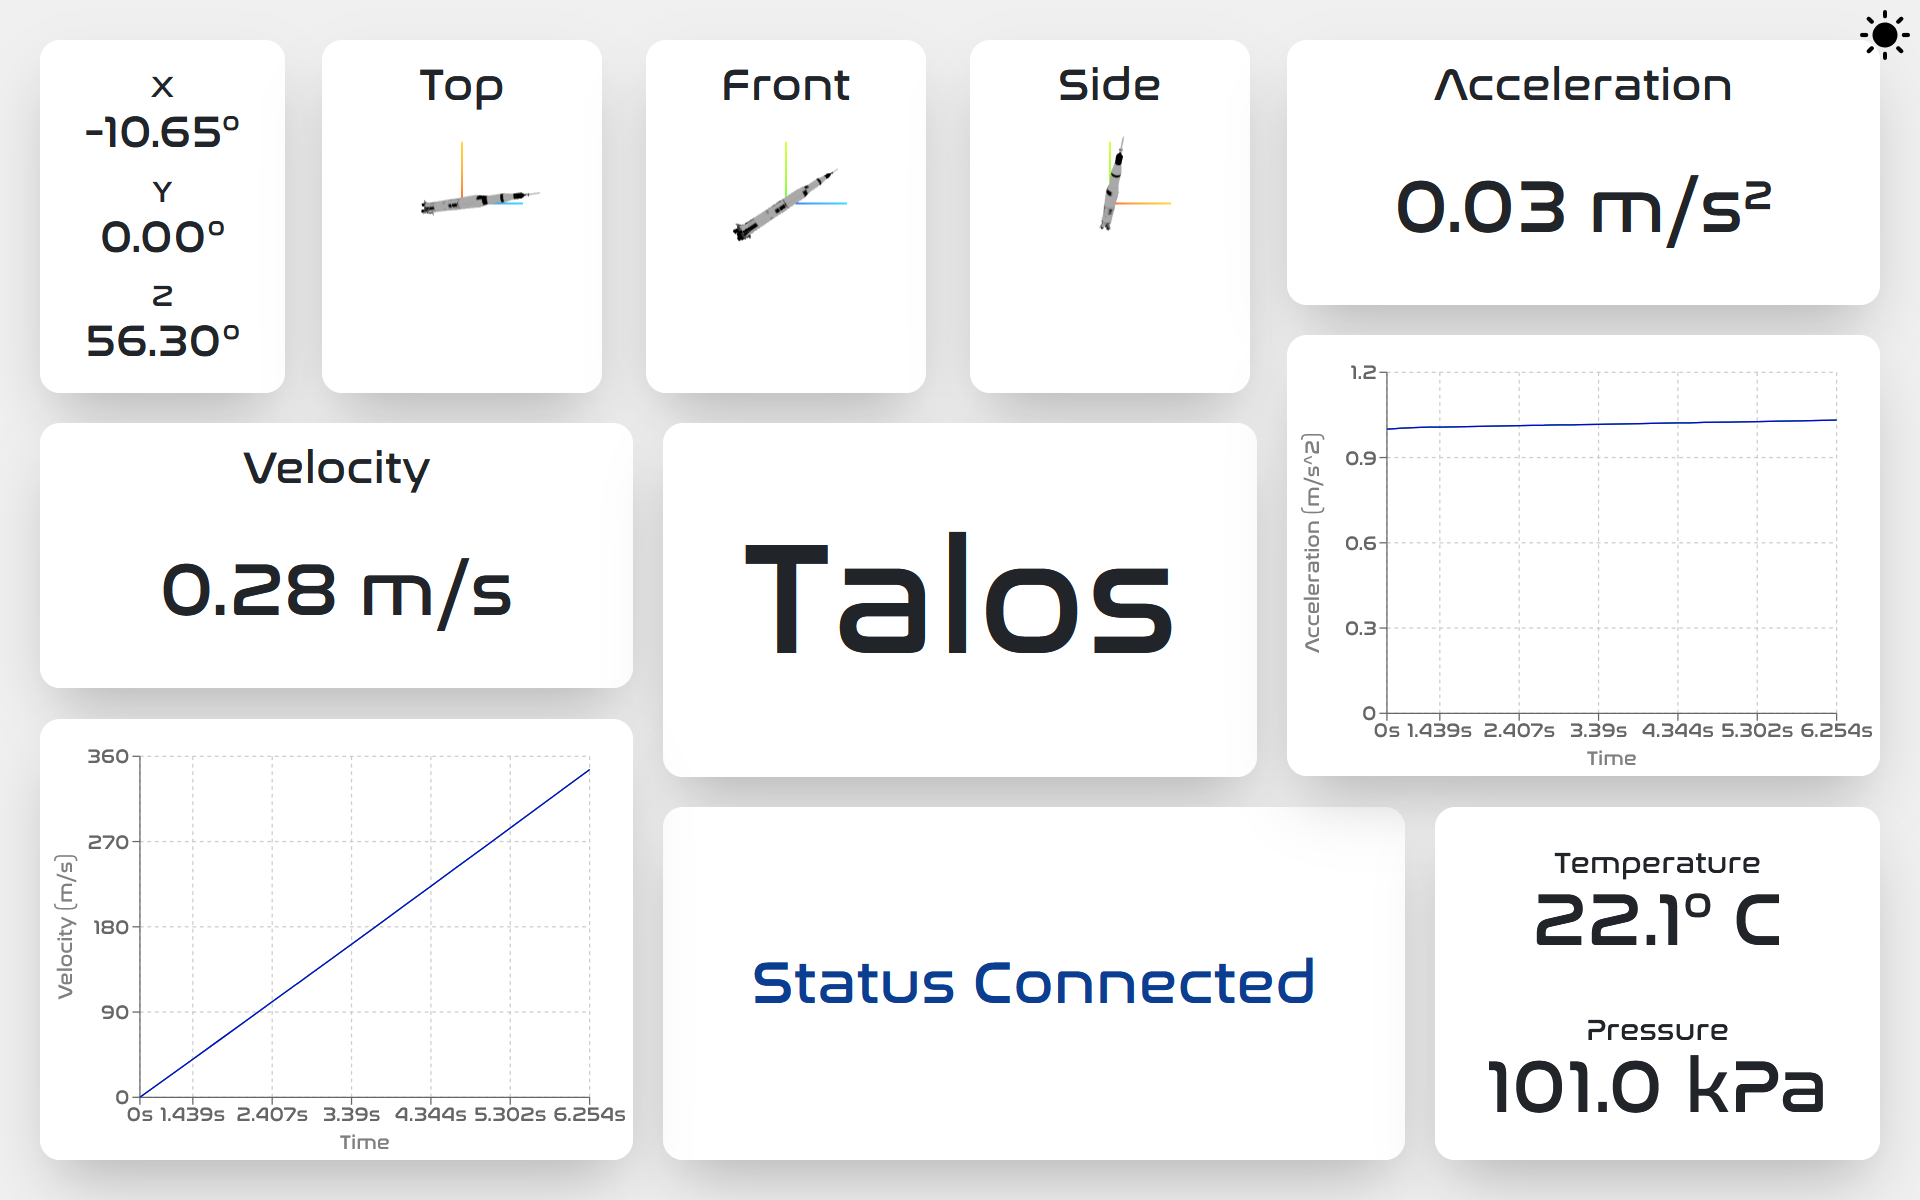
\includegraphics[width=\textwidth]{website_data.png}
\end{figure}
\subsubsection{Programming}
\qquad We then proceeded to program the board using the STM32CubeIDE, a free IDE provided by STMicroelectronics\cite{STM32CubeIDE}. We had to learn how to use the IDE, program the microcontroller, and interface with the sensors in the C programming language. We achieved this through open-source drivers that we ported to the STM32 MCU. We discovered another error after configuring all the drivers for the various sensors. In the BMP580, we forgot two more decoupling capacitors, which impeded the sensor from starting up. We are currently working on resolving this problem, as the soldering technique required to fix the issue is exact.
\subsection{Testing}
\qquad To test the board, we designed and created an interactive web page that would display the data from the sensors in real-time. We used the serial port to send the data through web sockets to a web server written in Rust. We chose Rust because of its speed and low memory usage, which are essential in any real-time application. We then used the WebSockets to send the data to the web page. We wrote the web page in React, Typescript, and TailwindCSS. We used React for the front end because of its ease of use and the ability to create interactive web pages. We used Typescript because of its type safety and the ability to catch errors at compile time. We used TailwindCSS for the styling because of its utility-first approach and the ability to create responsive designs. The web page displayed the data from the sensors in real-time, including the rocket's orientation, altitude, airspeed, and temperature. The website is shown in Figures \ref{fig:website_no_data} and \ref{fig:website_data}, and it can be accessed at \texttt{https://talos.notaroomba.dev}.

\section{Results}
\qquad After starting the project in August of 2024, we were surprised at how much we learned quickly. We learned how to design a PCB, program a microcontroller, and interface with sensors. We also learned to use tools and libraries like EasyEDA, STM32CubeIDE, Rust, C, and WebSockets. As it was our first time working on a project of this magnitude, we encountered many challenges. We had to learn how to read datasheets, troubleshoot errors, and work as a team. We are proud of our accomplishments and are excited to continue working on the project. Talos has the potential to inspire others to explore the exciting world of aerospace engineering and rocketry.

\section{Future Work}
\begin{itemize}
      \item Add a GPS module to the board to track the rocket's position.
      \item Add a magnetometer to the board to measure the rocket's orientation.
      \item Add a camera to the board to capture images and video of the rocket's flight.
      \item Redo the PCB layout and place the IMU sensor in the center of the board.
      \item Upgrade the sensors as new versions come out.
\end{itemize}
\printbibliography

\end{document}